\documentclass{article}
\usepackage[utf8]{inputenc}
\usepackage{csquotes}
\usepackage{booktabs}
\usepackage{multirow}
\usepackage{adjustbox}
\usepackage{tabularx}
\usepackage{array}
\usepackage{rotating}
\usepackage{float}

\title{Gesture Based User Interface Experience – Accessibility, Evolution and Challenges}
\author{William Vida}
\date{}

\usepackage{natbib}
\usepackage{graphicx}

\begin{document}

\maketitle

\section*{User Experience Evolution}
Today, the keyboard and mouse provide the majority of user input for computer systems. But there are other methods of user input including hand or other body gestures, eye tracking and console controllers \cite{bhuiyan2009gesture}. Microsoft's Kinect for the Xbox 360 is an example of a gesture-based system. The Kinect was controller free and allowed users to make hand and arm movements which were used as inputs instead of a controller for certain video games \cite{10.1007/978-3-642-34182-3_4}.

\begin{figure}[h!]
	\centering
	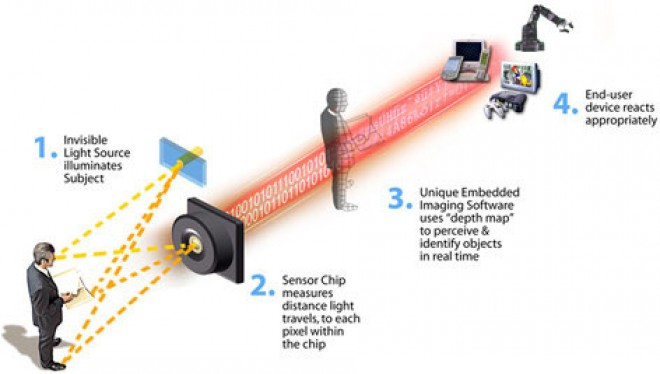
\includegraphics[width=1.0\linewidth]{images/depth-perception-using-the-infrared-camera.jpg}
	\caption{Depth perception using an infrared camera.}
	\label{fig:Depth perception using an infrared camera.}
\end{figure}

\begin{figure}[H]
	\centering
	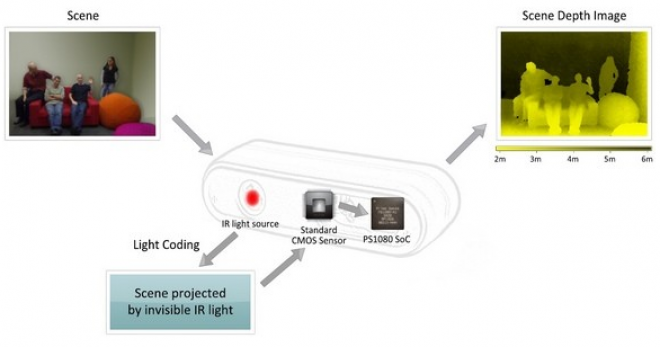
\includegraphics[width=1.0\linewidth]{images/transfer-of-information-from-the-camera-to-the-TV.png}
	\caption{Transfer of information from the camera to the TV.}
	\label{fig:Transfer of information from the camera to the TV.}
\end{figure}

The mouse was created in the early 1960s at the Stanford Research Institute by Douglas Engelbart. The mouse was originally meant to be a cheap replacement for light pens. Engelbart showed the uses of the mouse in a movie in 1968. Many of the uses shown in the movie are still used today. The mouse commercially appeared in products such as the Apple Lisa and the Xerox Star in the 1980s \cite{10.1145/274430.274436}.

\begin{figure}[H]
	\centering
	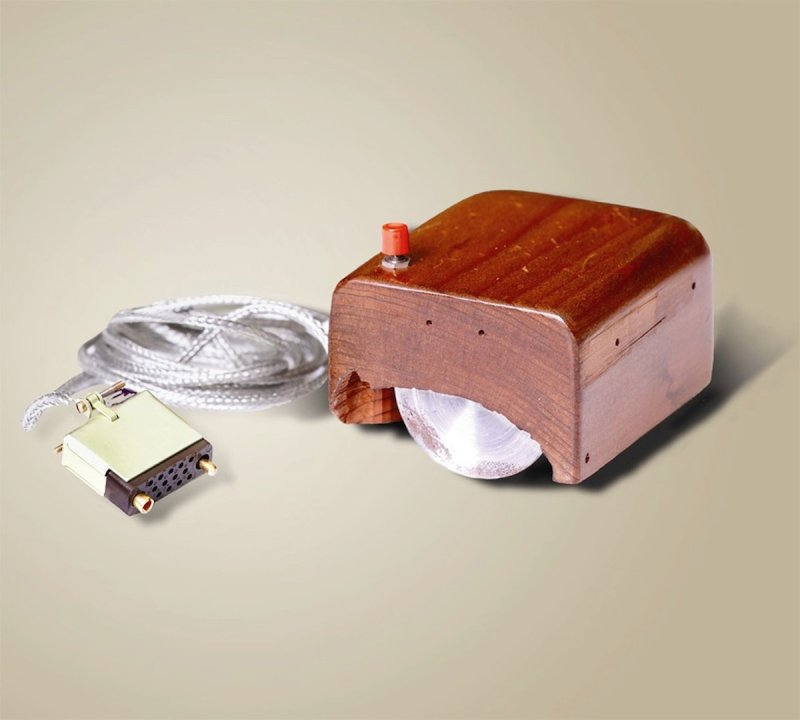
\includegraphics[width=0.45\linewidth]{images/the-first-mouse.jpeg}
	\caption{The first mouse.}
	\label{fig:The first mouse.}
\end{figure}

The first pen-based computer was the Rand Tablet which was developed by the Advanced Research Projects Agency (ARPA). The first trainable gesture recogniser was invented by Warren Teitelman in 1964. Tom Ellis used the Rand Tablet to create an early demo of gesture recognition called Graphic Input Language (GRAIL). It was very customary for light pen-based systems to provide gesture detection. Since the 1970s, gesture recognition has been used in industrial CAD systems \cite{10.1145/274430.274436}.

In recent years, gesture-based interaction has become an essential part of modern interfaces. This can be seen across multiple areas in our way of life including workplaces and entertainment. Gestures can include touch screen gestures and free form or in-air gestures. Touch screen interaction is done by touching a screen directly with one's fingers. While in air gestures are done by making a certain gesture with one's hand and/or fingers in front of a camera or a number of sensors. But, to use mid-air gestures a dedicated input device must be used which can include gloves or controllers, or the gestures executed must be done within a certain range of depth-sensing sensors or infrared sensors \cite{doi:10.1177/0018720818824253}.

Gesture-based input has advantages over normal input devices which can include naturalness and the ease of learning. Gesture-based input would preferably allow users to concentrate on the current task and not on the input device. Users can feel an increased sense of power and control when the computer reacts to gestures that are perceived to be natural. Users can also feel more personal identity and pleasure when using a system that reacts to their gestures \cite{10.1007/978-3-642-34182-3_4}.

Gesture-based input can help the elderly and those with disabilities. Due to changes in demographics, in the coming future, we will see more elderly people and less young people. This could mean that mouse and keyboard will be replaced by gesture-based applications for elderly people and also those with disabilities \cite{bhuiyan2009gesture}.

One area of gaming that has been on the rise in recent years is virtual reality. Virtual reality involves using a headset device strapped to ones face, motion controllers and of course a monitor and usually a powerful computer, to get a superior virtual reality gaming experience, in order to play. Virtual reality can add more immersion and intensity to one's gaming experience than a normal controller or keyboard and mouse can. Virtual reality gaming can "enhance[] overall satisfaction, enjoyment, engrossment, creativity, sound, and graphics quality". Steam, which is a digital video game marketplace, 16\% of video games available for sale there supported a virtual reality headset in 2016. And 83\% of those video games required a virtual reality headset in order to play \cite{shelstad2017gaming}.

\begin{figure}[H]
	\centering
	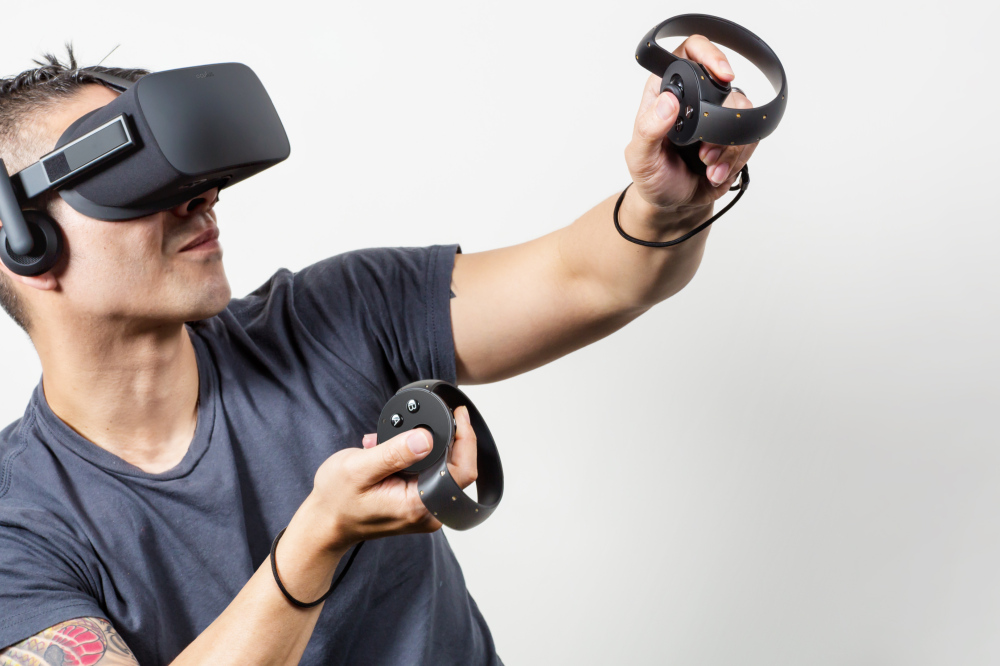
\includegraphics[width=0.72\linewidth]{images/oculus-touch.jpg}
	\caption{The Oculus Rift headset and the Oculus Touch motion controllers.}
	\label{fig:The Oculus Rift headset and the Oculus Touch motion controllers.}
\end{figure}

\section*{Gestures as a Communication Tool}
Hand gestures are just part of non-verbal communication channels. Gestures can be complex in part due to the fact that similar movements are used to send different types of messages. Gestures can be iconic or arbitrary, they can refer to objects or go hand in hand with the words of the speaker or they can be directed at themselves or to other people around the speaker. Speech is usually accompanied by changes to bodily movements in particular to the hands and face of the speaker. Those two have been found to be very highly linked with speech even down to the level of each syllable. An explanation for this proposes that language "evolved from gestures-first pointing at objects and animals, then representing animals by imitating their movements, and objects by the movements used to make or use them" \cite{https://doi.org/10.1080/00207597508247319}.

The frequency of gestures used along with speech can depend on the culture one person is in. For example, Italians are said to be a people where hand gestures are used very often and use them more than the English which is considered a low gesture usage people. But it must be said that it is unclear if Italians communicate more information by using hand gestures. Observed cultural differences in Italian and Jewish migrants to the United States showed different gestures by them. Italian migrants used more "kinetographs (showing a bodily action) and pictographs (drawing a picture)". Italian gesturing can also include sign language. British-Americans do not make their hand gestures as openly as Italian-Americans. British-American children are taught not to make gestures as it is seen as rude. There are individual differences when it comes to the capability to send and receive nonverbal signals but these differences have been shown to not be related. A study found that the ability to identify voice-tone emotions has a correlation with intelligence and with the ability to vocally express feelings \cite{https://doi.org/10.1080/00207597508247319}.

\begin{figure}[H]
	\centering
	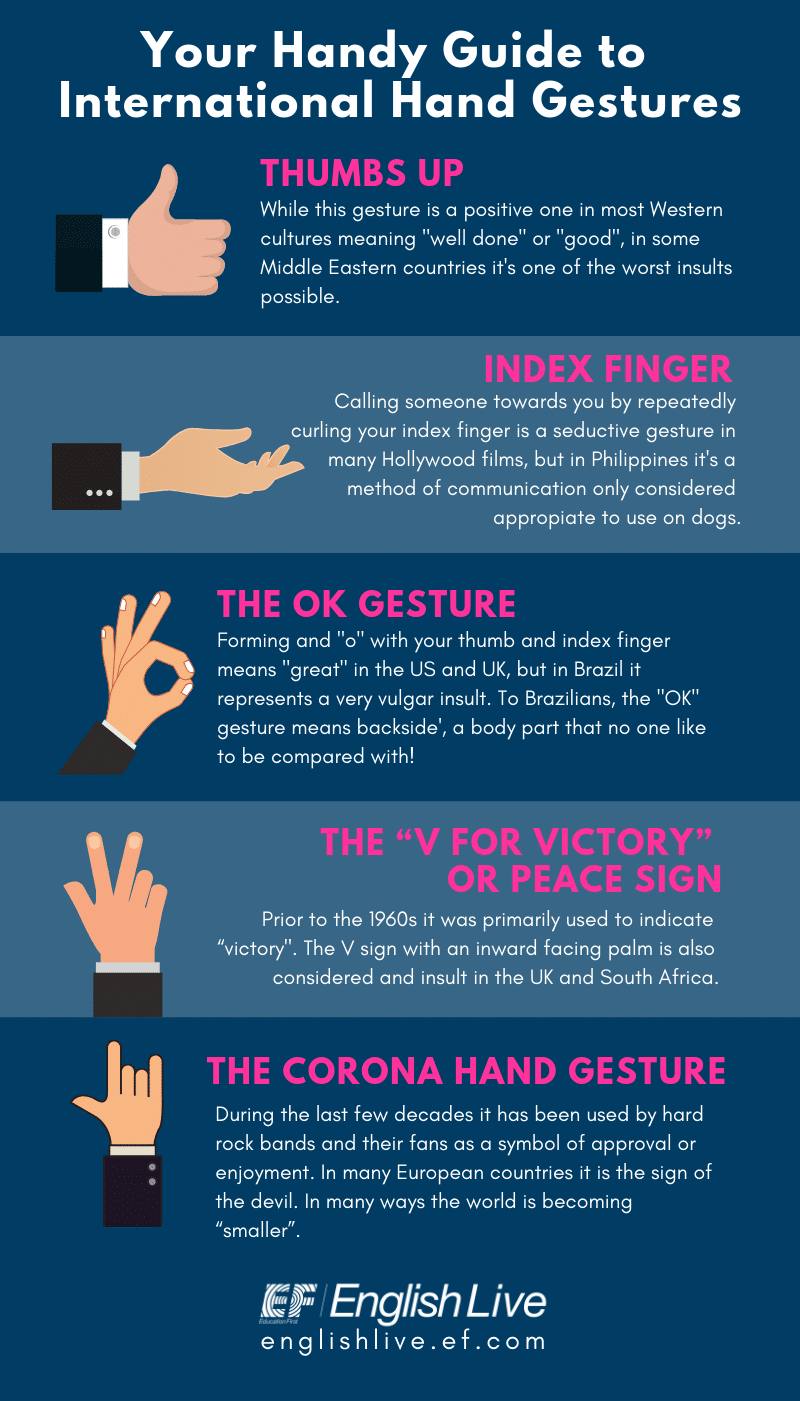
\includegraphics[width=0.6\linewidth]{images/some-hand-gestures.png}
	\caption{Some international hand gestures.}
	\label{fig:Some international hand gestures.}
\end{figure}

Gestures used during verbal communication have been found to have an information value that can be utilised by both speakers and listeners. For example, those who are also language learners use gestures as a means to provide verbal help when they interact with native listeners. An experiment was conducted where listeners were asked to repeat a story told to them by a speaker whose gestures did not always match the corresponding speech. The results showed that "information in the gestural channel is retained by the listeners and integrated with information from the spoken channel into what can be thought of as an intermodal cognitive representation of meaning" \cite{jbp:/content/journals/10.1075/pc.7.1.04gul}.

Face to face interaction is where most gestures take place. The listener in this case usually looks at the face of the speaker. Assuming this is followed, then gestures made would have to be taken in through one's peripheral vision. Research and analysis of gesture recognition, particularly in face-to-face conversation, have rarely had sufficient control over the visual perception of the listener but mostly relied on video recordings from the speaker's point of view \cite{jbp:/content/journals/10.1075/pc.7.1.04gul}.

Studies have shown that while speech is immersed in noise, gestures may increase language understanding, have a beneficial effect on future memory of the language information and may even serve as a disambiguation cue when speech is unclear or includes an uncertain term. A 2010 study, proposed the integrated-systems hypothesis which states the usage of gesture and speech is mutual and compulsory. This means that gestures are always taken into consideration and one cannot circumvent using them in a speech \cite{OBERMEIER2012857}.

\begin{figure}[H]
	\centering
	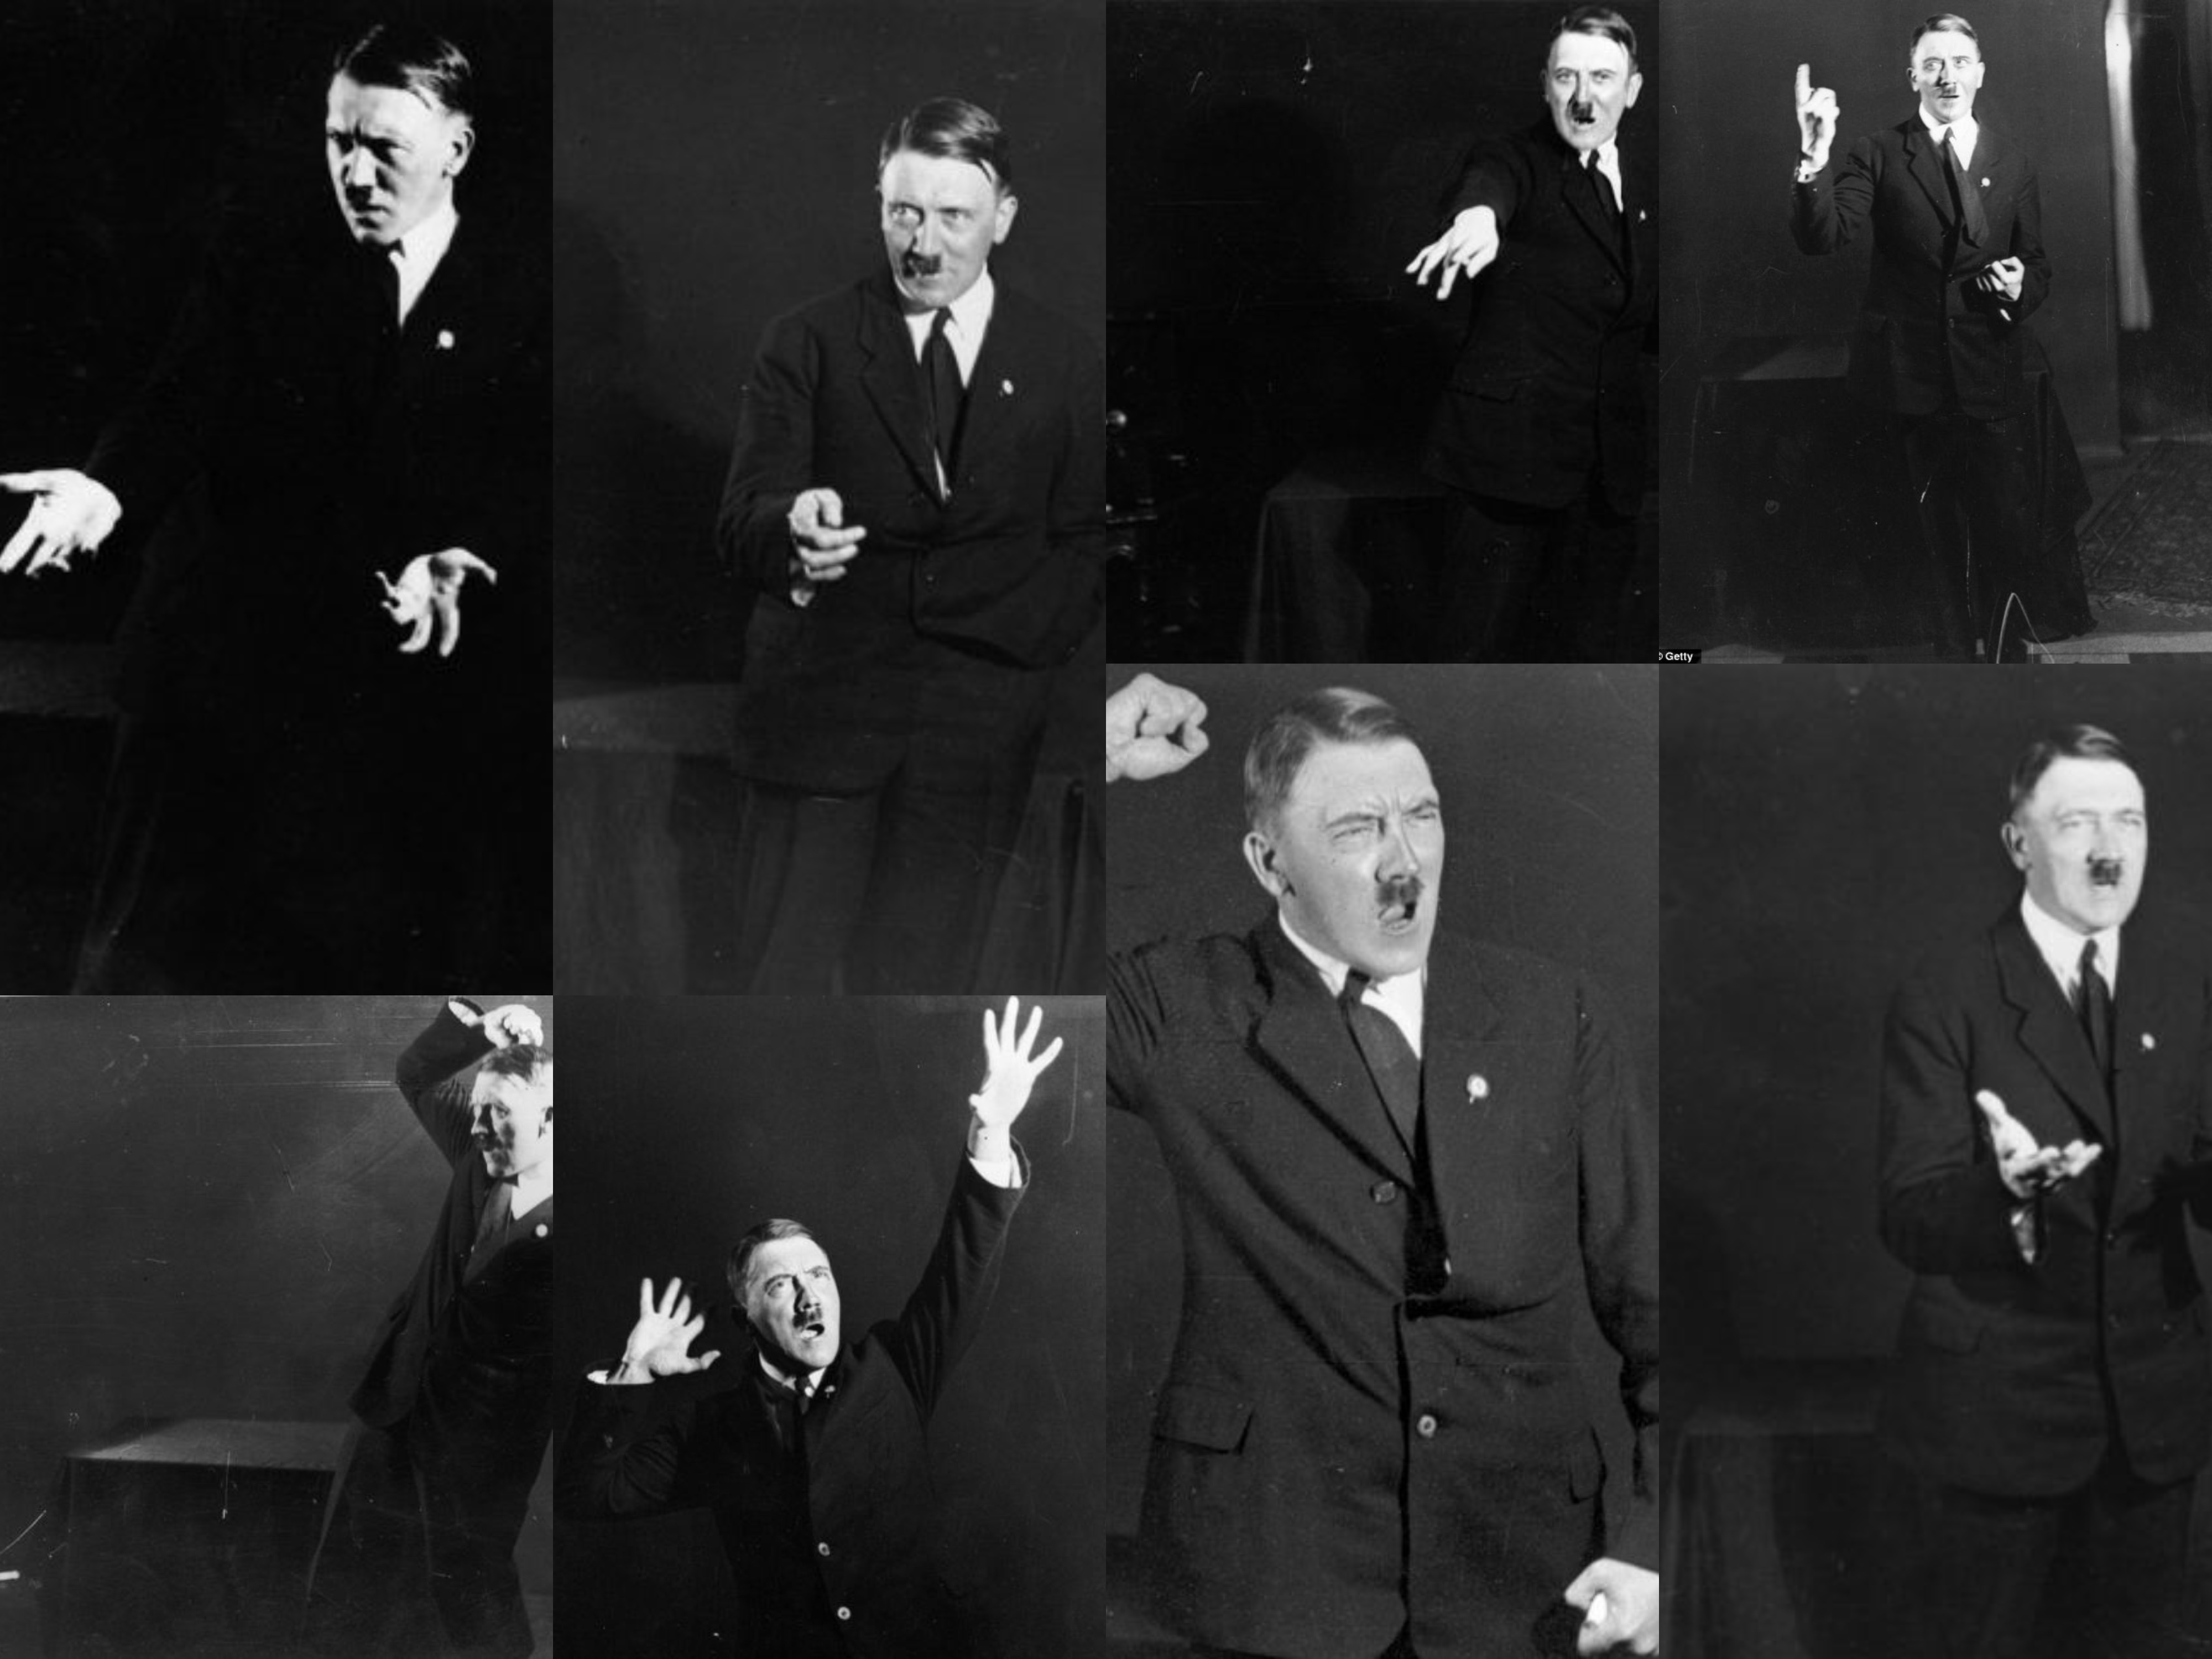
\includegraphics[width=0.8\linewidth]{images/adolf-hitler-practising-hand-gestures.jpg}
	\caption{Adolf Hitler practising his hand gestures for his speeches. Reportedly taken in 1925.}
	\label{fig:Adolf Hitler practising his hand gestures. Reportedly taken in 1925.}
\end{figure}

A 2004 study explored the effects of gestures on language comprehension. The study recorded event‐related potentials (ERPs) which are "electrophysiological neural responses time-locked to a
stimulus \cite{https://doi.org/10.1111/1460-6984.12535}", elicited by spoken words said at the same time with gestures that either agreed with the words spoken or disagreed with the words spoken. Stimuli were made by recording an actor while the actor was gesturing to either a tall, thin glass and a short, wide dish. The actor said one of the following speech tokens, tall and thin (the glass) and short and wide (the dish). The matching condition involved the speech made by the actor matching with both the object described in the speech as well as the same dimension (the actor said the tall and gestured the height of the tall, thin glass). The mismatch involved the speech token matching to one object while the gesture matched to the other. When there was no gesture condition the speech was presented alone \cite{WU2007234}. The results showed that:
\begin{quote}
	Early effects of gesture congruency (between 100 and 352 ms), with mismatching and complementary stimuli eliciting relative to other conditions larger P1 and P2 components, which reflect auditory sensory processing. N400-like effects were also observed at bilateral temporal electrode sites, with mismatch trials eliciting more negative ERPs than all other conditions around 450 ms post-stimulus. These findings suggest that gesture congruency affects both early sensory as well as higher order semantic processing of words \cite{WU2007234}.
\end{quote}

\section*{Challenges for Design of Applications}
For many human-computer interaction systems, hand gesture movement seems to be the most natural and appropriate as it is similar to how humans interact with each other. One suggestion is to use a virtual mouse. There is a sizeable market for hand gestures systems and there remain challenges for the development of hand gesture recognition systems. A virtual mouse can replace the use of a physical keyboard and mouse but this still has problems that need to be sorted out. Hand gesture recognition is a key issue that needs to be tackled when designing a virtual mouse device. A very effective form of equipment for recording hand gesture movement is through electromechanical or magnetic sensing devices (data gloves). This process uses sensors attached to a glove that converts finger movements into electrical signals to recognise hand gestures. Data gloves that are used with hand gestures have been used in sign language analysis and training and to control robotic arms. Unfortunately, data gloves have many drawbacks. These include that due to their complexity their costs remain high. The size of data gloves can also cause issues. This makes it difficult to use data gloves for day to day activities. Vision-based gesturing provides a very hopeful alternative to data gloves as it is non-contact and feels more natural than data gloves. Vision-based gesturing is based on computer vision algorithms. Algorithms are used for hand segmentation based on a background model. Colour-based algorithm systems are used to distinguish the area of the object of interest. Hand gesture identification helps increase precision when analysing a vast amount of hand gestures \cite{tsai2020design}.

\begin{figure}[H]
	\centering
	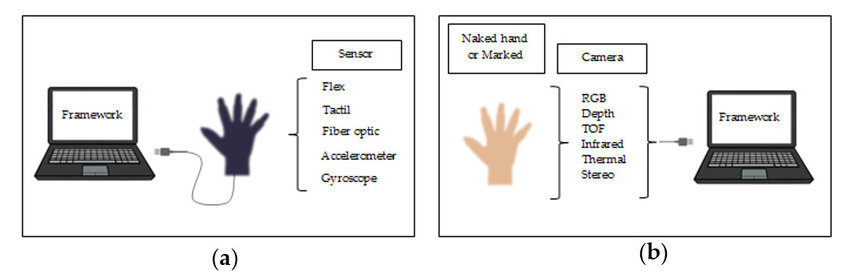
\includegraphics[width=1.0\linewidth]{images/different-techniques-for-hand-gestures-a-Glove-based-attached-sensor-either-connected.png}
	\caption{Two different techniques for hand gestures showing a glove sensor and mid-air hand gestures.}
	\label{fig:Two different techniques for hand gestures showing a glove sensor and mid-air hand gestures.}
\end{figure}

It can be difficult to achieve a high hand gesture recognition accuracy when having complex backgrounds, changes to the external lighting and shadows of the hand gestures. It was suggested to use RGB cameras to detect hands but it was hard to use in certain lighting conditions and for different skin colours. It was better to use depth cameras to differentiate hands in front of a camera. A study found that when hand gestures contained a background, a human face and a human body, the accuracy for detecting hand gestures was 97.1\% with a simple background while the accuracy dropped to 85.3\% when a complex background was in place. Tests were done using a Kinect to show that if there is a larger object than a hand then the gestures made will be inaccurately analysed by the Kinect. A deep learning neural network was made which analysed a large set of computer-generated 3D hand images with some real camera images as part of the training data set. The testing and training data sets for both had 24 classes of hand gestures and the hand gesture accuracy was 77.08\% \cite{yasen2019systematic}.

Study gaps can be easy to find in the field of hand gesture recognition systems as research studies tend to focus on computer applications, sign language, and interacting with a 3D model in a simulated environment. However, numerous scientific papers are concerned with strengthening the system for hand gesture recognition or designing new algorithms rather than applying a realistic application with respect to healthcare. A big challenge researchers face is to design a functional system that overcomes the most common problems with fewer constraints and produces precise and consistent performance \cite{jimaging6080073}.

Many of the hand gesture systems that are suggested can be placed into two different categories of computer vision techniques. The first one is to use image processing methods by either using Open-NI libraries or OpenCV libraries and other resources if necessary to provide real-time interaction that recognises time consumption due to real-time processing. This has drawbacks which can include "backdrop problems, lighting changes, distance restrictions, and multi-object or multi-gear issues". The second category involves using gestures contained in data sets to match the gestures made by the user where significantly more complicated patterns need more advanced algorithms. Artificial intelligence and deep learning methods can be used to recognise a vast number of gestures in real-time by analysing gestures in a data set containing specific postures or gestures. This method does have issues which can include overlooking some gestures due to the accuracy contrast of the classification algorithm \cite{jimaging6080073}.

When designing hand gesture systems, the designers must take into account the differences in hand gestures in different nations and different cultures. Certain hand gestures can have different meanings around the world. A gesture that is positive or neutral in one country might be considered offensive or insulting in another one even if they were unintentional. People who are not from the countries of the designers of hand gesture systems might move their hands in a different way than the way the system was designed for which could reduce the precision of the hand gesture recognition system. A study was done using 54 Lao alphabets while four individuals did 540 gestures. The camera had difficulty in keeping up with the speed of the hand gestures and it had an accuracy rate of 79\% \cite{shanthakumar2020design}.

\section*{Challenges for Implementation}
Hand gesture user interfaces should be able to perform gesture recognition at high accuracy in real-time. Those systems should be able to detect hands, track their movement and the gestures they make. Tracking describes the process of following the user's hands frame by frame. Detecting hands can be difficult as there can be a high variation in one's hand shape and size, skin colour and the lighting condition the user is in. Tracking issues can happen if there are tight spaces, a cluttered environment and quick hand movements. When deploying a hand gesture system it can be difficult for everyday environments. The camera sensor and lens, the background and the differences of the user can make rolling out the product difficult \cite{10.1145/1897816.1897838}.

The recognition of hand gestures includes complex processes such as motion modelling, motion analysis, pattern recognition and machine learning. The environmental background of the user such as background lighting and the speed of the movement affects the tracking and the accuracy of the prediction. Anticipated problems that can arise include "temporal variance, spatial complexity, movement epenthesis, repeatability and connectivity as well as multiple attributes such as change of orientation and region of gesture carried out". Criteria to judge gesture recognition systems include "scalability, robustness, real-time performance and user-independent" \cite{cheok2019review}.

Virtual reality has potential but currently, it has some drawbacks and a big one includes cybersickness. Symptoms of cybersickness can include "headaches, eyestrain, stomach awareness, and nausea, sometimes severe enough to result in vomiting". Cybersickness is similar to motion sickness but the main difference is that motion sickness occurs when "actual physical bodily motion does not match what is perceived visually". A lot of research has been done to find the causes and to avoid cybersickness when using virtual reality equipment. There was very little difference between the first generation of the Oculus Rift DK1 and its successor the DK2 when it came to cybersickness \cite{shafer2019factors}. The market for virtual reality is quite small compared to other forms of gaming such as console and PC gaming. This means that there is a lack of games for virtual reality and a lack of games that are of good quality. There a few reasons for this, one is because that virtual reality is a new technology and it takes more time for developers to develop and test these games. Another is that virtual reality equipment is expensive. Virtual reality headsets can cost more than \$500 and one would also need a powerful computer to run these games. And one would, of course, need space to play the games as well \cite{shelstad2017gaming}.

\section*{Conclusions}
Hand gestures are used very often when people talk to each other or when giving a speech. They can help make one person a better speaker and allows them to connect to whom you are talking to better. Audiences feel more connected if a speaker is making hand gestures than one who is inactive.

The ways for using computers have evolved but the mouse and keyboard remain the dominate methods used for human interaction with computers to this day even after a few decades after their invention. Phones have evolved from needing a number pad to being completely touch screen in less than 15 years. There have been attempts to bring hand gestures into video games with the Kinect being the most famous but even though it seemed to be revolutionary at the time, the Kinect was arguably a failure for Microsoft. Virtual reality video games remain an expensive alternative to the usual keyboard and mouse for gaming but a problem with virtual reality is that they lack dedicated games as most of the PC gaming market is with keyboard and mouse. This is not to say that there never will be a market for hand gestures interfaces. They seem to be more useful in other fields but maybe as technology advanced they might make another rise in gaming. Hand gesture technology is advancing quickly and maybe within a few decades or less they will be commonplace in our daily lives. Hand gesture technology has advantages such as it being controller/mouse and keyboard free and no set up is required other than a camera. But as mentioned it may be a long time until they are mainstream.

\bibliographystyle{plain}
\bibliography{references}

\end{document}
